\documentclass[a4paper, 12pt]{article}

\usepackage{amsmath}
\usepackage{amssymb}
\usepackage{graphicx}
\usepackage{listings}[language=Python]
\lstdefinestyle{mystyle}{
    breakatwhitespace=false,         
    breaklines=true,                 
    captionpos=b,                    
    keepspaces=true,                 
    numbers=left,                    
    numbersep=5pt,                  
    showspaces=false,                
    showstringspaces=false,
    showtabs=false,                  
    tabsize=2
}

\lstset{style=mystyle}

\title{Lab-03 Report}
\author{st122246}

\begin{document}
	\maketitle

	\section{Chessboard calibration}
	\subsection{Save the image of chessboard for use in camera}

	% \begin{figure}
	% 	\caption{Save Chessboard image}
	% 	\includegraphics[]{}
	% \end{figure}
	
	main.py
	\begin{lstlisting}
import cv2 as cv

video_capture = cv.VideoCapture()
video_capture.open(0, cv.CAP_ANY)
if not video_capture.isOpened():
    print("ERROR! Unable to open camera\n")
    exit()

print("Start grabbing")
print("Press s to save images and q to terminate")

frame_add = 0
while True:
    _, frame = video_capture.read()
    if frame is None:
        print("ERROR! Blank frame grabbed\n")
        exit()

    cv.imshow("Live", frame)

    iKey = cv.waitKey(5)
    if iKey == ord('s') or iKey == ord('S'):
        cv.imwrite("../../../Data/Lab03/images/frame" + str(frame_add) + ".jpg", frame)
        frame_add += 1
        print("Frame: ", frame_add, " has been saved.")
    elif iKey == ord('q') or iKey == ord('Q'):
        break
	\end{lstlisting}


	\subsection{Camera Calibration}

	\begin{figure}
		\caption{1.2 Checkerboard Corners}
		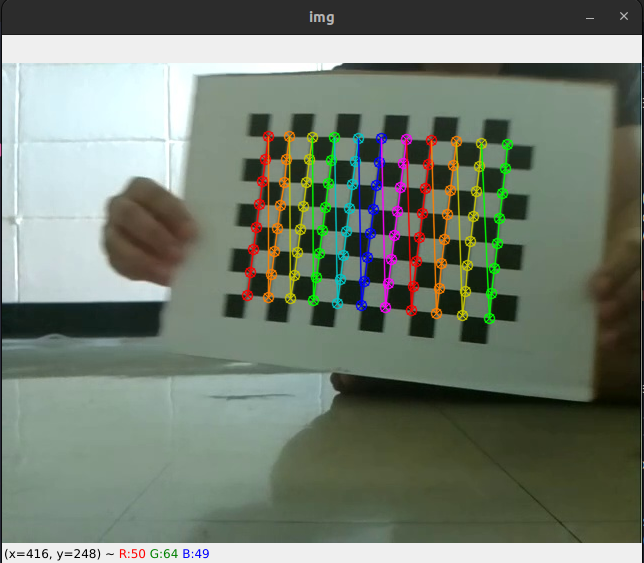
\includegraphics[scale=0.6]{images/checkerboard_corners.png}
	\end{figure}

	\begin{figure}
		\caption{1.2 Camera Matrix and Distortion Coefficient}
		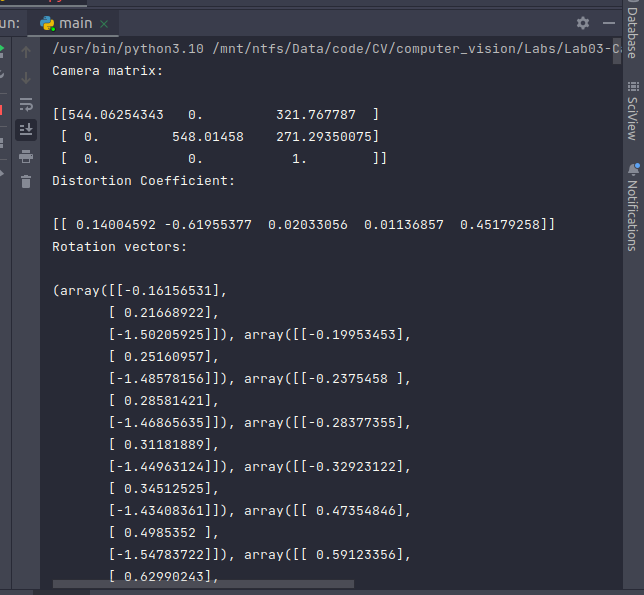
\includegraphics[scale=0.6]{images/cam_mtx_dist_coe.png}
	\end{figure}
	
	\begin{figure}
		\caption{1.2 Result}
		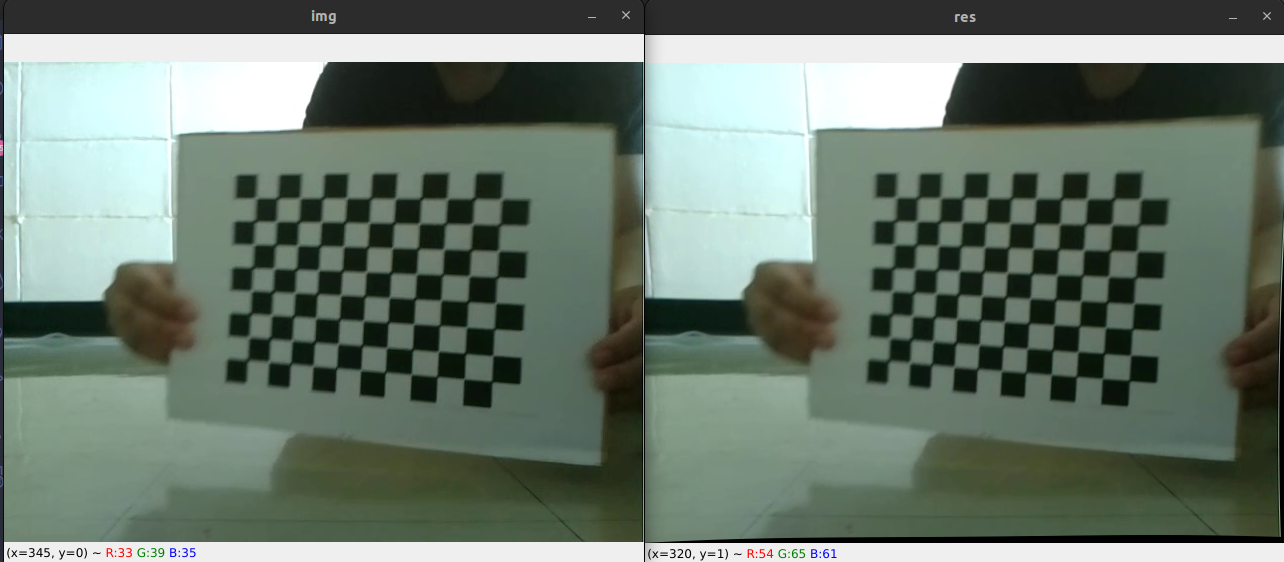
\includegraphics[scale=0.3]{images/refined_result.png}
	\end{figure}
	
	\begin{figure}
		\caption{1.2 Re-projection Error}
		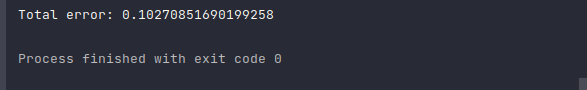
\includegraphics[scale=0.65]{images/reprojection_error.png}
	\end{figure}

	main.py
	\begin{lstlisting}
import glob
import cv2 as cv
import numpy as np


# Define the dimensions of checkerboard
CHECKERBOARD = (8, 11)
criteria = (cv.TERM_CRITERIA_EPS + cv.TERM_CRITERIA_MAX_ITER, 30, 0.001)

# Create vector to store vectors of 3D points for each checkerboard image
obj_points = []
# Create vector to store vectors of 2D points for each checkerboard image
img_points = []

# Define the world coordinates for 3D points
obj_point = np.zeros((1, CHECKERBOARD[0] * CHECKERBOARD[1], 3), dtype=np.float32)
obj_point[0, :, :2] = np.mgrid[0:CHECKERBOARD[0], 0:CHECKERBOARD[1]].T.reshape(-1, 2)
prev_img_shape = None

# Extracting path of individual image stored in a given directory
images = glob.glob("../../../Data/Lab03/images/*.jpg")
img = None
gray = None
for f_name in images:

    img = cv.imread(f_name)
    gray = cv.cvtColor(img, cv.COLOR_BGR2GRAY)

    # Find the chessboard corners
    # If desired number of corners are found in the image then ret = true
    ret, corners = cv.findChessboardCorners(gray, CHECKERBOARD, cv.CALIB_CB_ADAPTIVE_THRESH + cv.CALIB_CB_FAST_CHECK
                                            + cv.CALIB_CB_NORMALIZE_IMAGE)
    """
        If desired number of corner are detected, refine the pixel coordinates and display them 
        on the images of checkerboard
    """
    if ret:
        obj_points.append(obj_point)

        # Refining pixel coordinates for given 2D points.
        corners2 = cv.cornerSubPix(gray, corners, (11, 11), (-1, -1), criteria)

        img_points.append(corners2)

        # Draw and display the corners
        img = cv.drawChessboardCorners(img, CHECKERBOARD, corners2, ret)
    cv.imshow('img', img)
    cv.waitKey(0)

cv.destroyAllWindows()

h, w = img.shape[:2]
"""
    Performing camera calibration by passing the value of known 3D points (obj_points) and 
    corresponding pixel coordinates of the detected corners (img_points)
"""
ret, mtx, dist, r_vectors, t_vectors = cv.calibrateCamera(obj_points, img_points, gray.shape[::-1], None, None)

print("Camera matrix: \n")
print(mtx)
print("Distortion Coefficient: \n")
print(dist)
print("Rotation vectors: \n")
print(r_vectors)
print("Translation vectors: \n")
print(t_vectors)

# Show images of undistorted
for f_name in images:
    img = cv.imread(f_name)
    res = cv.undistort(img, mtx, dist)
    cv.imshow('img', img)
    cv.imshow('res', res)
    cv.waitKey(0)

# Use ROI obtained above to crop the result
print("Undistorted using ROI")
for f_name in images:
    print(f_name)

    img = cv.imread(f_name)

    h, w = img.shape[:2]
    new_camera_mtx, roi = cv.getOptimalNewCameraMatrix(mtx, dist, (w, h), 1, (w, h))
    res = cv.undistort(img, mtx, dist)

    # crop the image
    x, y, w, h = roi
    res = res[y:y+h, x:x+w]

    cv.imshow('img', img)
    cv.imshow('res', res)
    cv.waitKey(0)


# Find a mapping function from the distorted image to undistorted image.
# Then use the remap function.
print("Find mapping from distorted to undistorted image.\nThen use the remap function.")
for f_name in images:
    print(f_name)

    img = cv.imread(f_name)
    h, w = img.shape[:2]
    new_camera_mtx, roi = cv.getOptimalNewCameraMatrix(mtx, dist, (w, h), 1, (w, h))

    map_x, map_y = cv.initUndistortRectifyMap(mtx, dist, None, new_camera_mtx, (w, h), 5)
    res = cv.remap(img, map_x, map_y, cv.INTER_LINEAR)

    # Crop the image
    x, y, w, h = roi
    res = res[y:y+h, x:x+w]

    cv.imshow('img', img)
    cv.imshow('res', res)
    cv.waitKey(0)

mean_error = 0
for i in range(len(obj_points)):
    img_points2, _ = cv.projectPoints(obj_points[i], r_vectors[i], t_vectors[i], mtx, dist)
    error = cv.norm(img_points[i], img_points2, cv.NORM_L2) / len(img_points2)
    mean_error += error
print(f"Total error: {mean_error / len(obj_points)}")

	\end{lstlisting}

	\section{Exercises}
	\subsection{Read and write calibration file}


	\begin{figure}
		\caption{2.1 Camera Calibration File}
		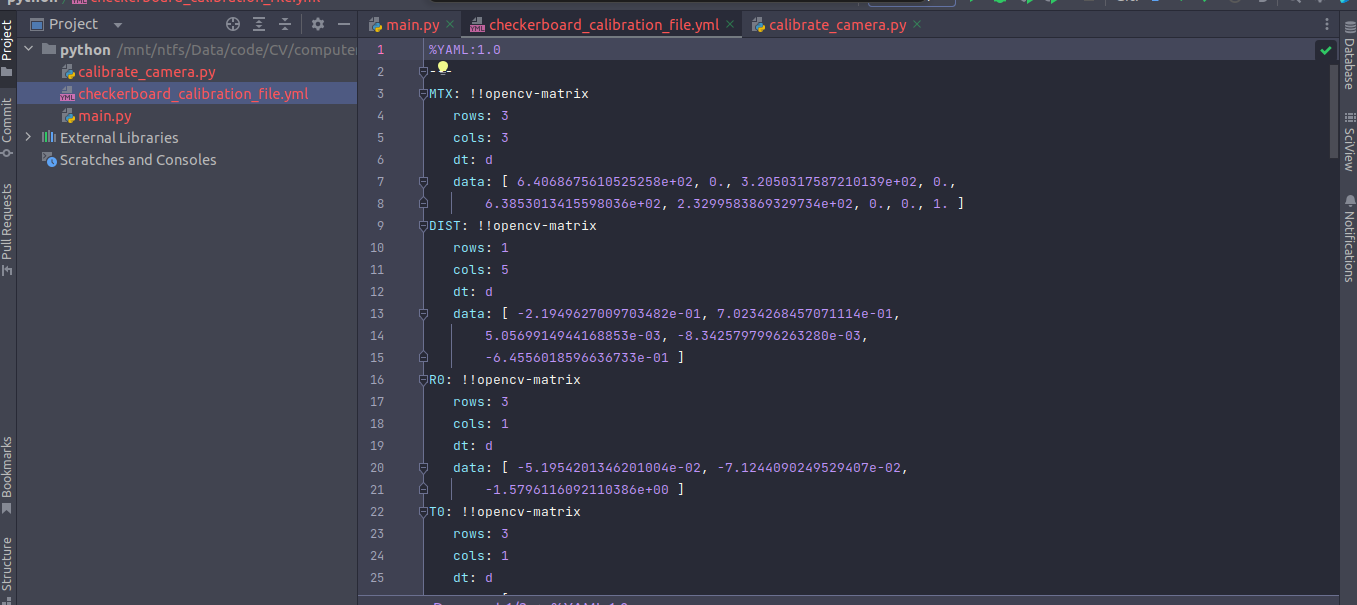
\includegraphics[scale=0.25]{images/camera_calibration_file.png}
	\end{figure}

	\begin{lstlisting}
# main.py
from calibrate_camera import CameraCalibration

camera_calibration = CameraCalibration()

camera_calibration.calibrate("../../../../Data/Lab03/images/")
print("Camera matrix: ", camera_calibration.camera_mtx)
print("Distortion coefficient: ", camera_calibration.distortion_coefficient)
print("Rotation vectors: ", camera_calibration.rotation_vectors)
print("Translation vectors: ", camera_calibration.translation_vectors)

camera_calibration.write_calibration_file("checkerboard_calibration_file.yml")
print()

camera_calibration.read_calibration_file("checkerboard_calibration_file.yml")
print("Camera matrix: ", camera_calibration.camera_mtx)
print("Distortion coefficient: ", camera_calibration.distortion_coefficient)
print("Rotation vectors: ", camera_calibration.rotation_vectors)
print("Translation vectors: ", camera_calibration.translation_vectors)
	\end{lstlisting}

	\begin{lstlisting}
# calibrate_camera.py
import glob
import cv2 as cv
import numpy as np


class CameraCalibration:
    camera_mtx = None
    distortion_coefficient = None
    rotation_vectors = None
    translation_vectors = None

    # Define the dimensions of checkerboard
    __CHECKERBOARD = (8, 11)
    __criteria = (cv.TERM_CRITERIA_EPS + cv.TERM_CRITERIA_MAX_ITER, 30, 0.001)

    # Create vector to store vectors of 3D points for each checkerboard image
    __obj_points = []

    # Create vector to store vectors of 2D points for each checkerboard image
    __img_points = []

    # Define the world coordinates for 3D points
    __obj_point = np.zeros((1, __CHECKERBOARD[0] * __CHECKERBOARD[1], 3), dtype=np.float32)
    __obj_point[0, :, :2] = np.mgrid[0:__CHECKERBOARD[0], 0:__CHECKERBOARD[1]].T.reshape(-1, 2)
    __prev_img_shape = None

    __img = None
    __gray = None

    def __init__(self, file_name=None):
        if file_name is not None:
            self.read_calibration_file(file_name)

    def calibrate(self, file_path):
        images = glob.glob(file_path + "*.jpg")

        for f_name in images:
            self.__img = cv.imread(f_name)
            self.__gray = cv.cvtColor(self.__img, cv.COLOR_BGR2GRAY)

            # Find the checkerboard corners
            ret, corners = cv.findChessboardCorners(self.__gray, self.__CHECKERBOARD, cv.CALIB_CB_ADAPTIVE_THRESH
                                                    + cv.CALIB_CB_FAST_CHECK + cv.CALIB_CB_NORMALIZE_IMAGE)

            # If the desired number of corner are detected
            if ret:
                self.__obj_points.append(self.__obj_point)

                # Refining pixel coordinates for given 2D points.
                corners2 = cv.cornerSubPix(self.__gray, corners, (11, 11), (-1, -1), self.__criteria)

                self.__img_points.append(corners2)

                # Draw and display the corners
                self.__img = cv.drawChessboardCorners(self.__img, self.__CHECKERBOARD, corners2, True)

            cv.imshow('img', self.__img)
            cv.waitKey(0)
        cv.destroyAllWindows()

        # Calibrate the camera
        ret, self.camera_mtx, self.distortion_coefficient, self.rotation_vectors, self.translation_vectors = \
            cv.calibrateCamera(self.__obj_points, self.__img_points, self.__gray.shape[::-1], None, None)

    def write_calibration_file(self, file_name):
        file_storage = cv.FileStorage(file_name, cv.FILE_STORAGE_WRITE)

        if not file_storage.isOpened():
            return False

        file_storage.write("MTX", self.camera_mtx)
        file_storage.write("DIST", self.distortion_coefficient)
        for i in range(10):
            file_storage.write("R" + str(i), self.rotation_vectors[i])
            file_storage.write("T" + str(i), self.translation_vectors[i])
        file_storage.release()

        return True

    def read_calibration_file(self, file_name):
        file_storage = cv.FileStorage(file_name, cv.FILE_STORAGE_READ)
        if not file_storage.isOpened():
            return False

        self.camera_mtx = file_storage.getNode("MTX").mat()
        self.distortion_coefficient = file_storage.getNode("DIST").mat()
        r_vectors = tuple()
        t_vectors = tuple()
        for i in range(10):
            r_vectors += (file_storage.getNode("R" + str(i)).mat(),)
            t_vectors += (file_storage.getNode("T" + str(i)).mat(),)
        self.rotation_vectors = r_vectors
        self.translation_vectors = t_vectors
        file_storage.release()

        return True
	\end{lstlisting}

	\subsection{Calibrate camera, re-calculate homography from own video}
	
	\begin{figure}
		\caption{2.2 Results on own video}
		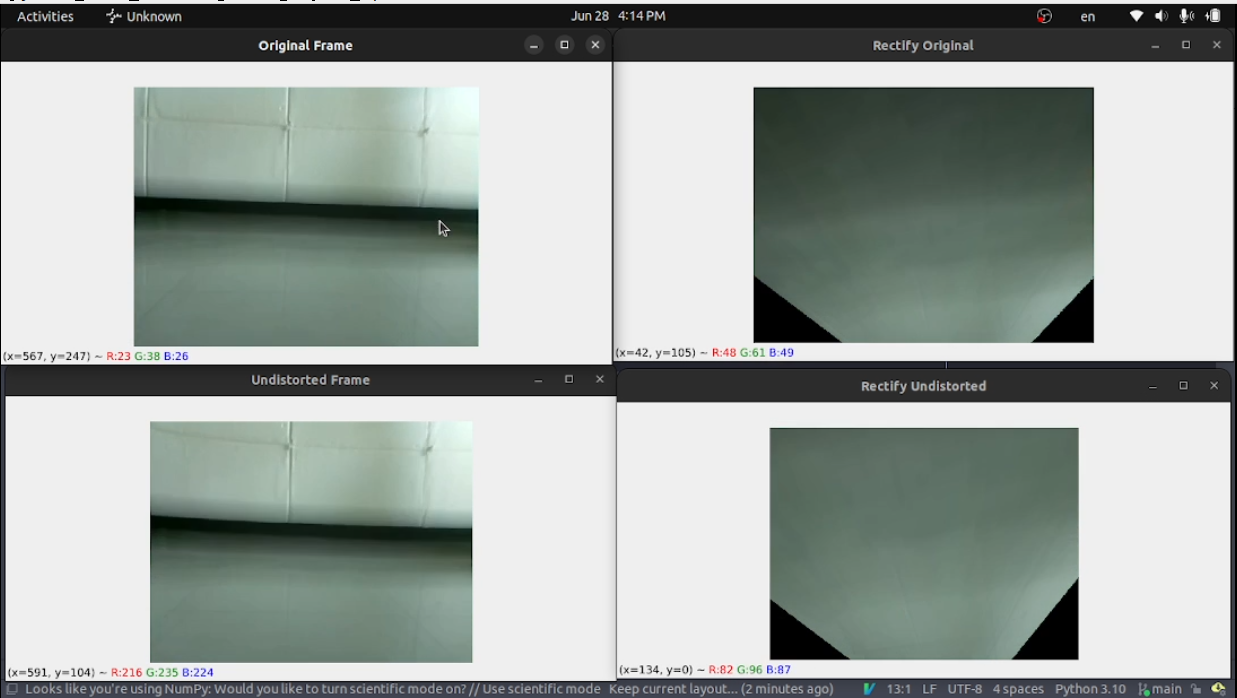
\includegraphics[scale=0.3]{images/own_video_result.png}
	\end{figure}

	\begin{lstlisting}
# capture_video.py
import cv2 as cv


def capture_video(file_name: str):
    video_capture = cv.VideoCapture(0)

    fourcc = cv.VideoWriter_fourcc(*"mp4v")
    out = cv.VideoWriter(file_name, fourcc, 20.0, (640, 480))

    while True:
        ret, frame = video_capture.read()

        out.write(frame)

        cv.imshow("Web Camera", frame)

        if cv.waitKey(30) & 0xFF == ord('q'):
            break

    cv.destroyAllWindows()
    video_capture.release()
    out.release()


def convert_video_to_images(file_name: str, path: str):
    video_capture = cv.VideoCapture(path + file_name)

    count = 0
    while True:
        ret, frame = video_capture.read()
        if frame is None:
            break
        cv.imwrite(path + "images/frame%d.jpg" % count, frame)

        count += 1

        cv.waitKey(30)

	\end{lstlisting}

	\begin{lstlisting}
# calibrate_camera.py	
import glob
import cv2 as cv
import numpy as np


class CameraCalibration:
    camera_mtx = None
    distortion_coefficient = None
    rotation_vectors = None
    translation_vectors = None

    # Define the dimensions of checkerboard
    __CHECKERBOARD = (8, 11)
    __criteria = (cv.TERM_CRITERIA_EPS + cv.TERM_CRITERIA_MAX_ITER, 30, 0.001)

    # Create vector to store vectors of 3D points for each checkerboard image
    __obj_points = []

    # Create vector to store vectors of 2D points for each checkerboard image
    __img_points = []

    # Define the world coordinates for 3D points
    __obj_point = np.zeros((1, __CHECKERBOARD[0] * __CHECKERBOARD[1], 3), dtype=np.float32)
    __obj_point[0, :, :2] = np.mgrid[0:__CHECKERBOARD[0], 0:__CHECKERBOARD[1]].T.reshape(-1, 2)
    __prev_img_shape = None

    __img = None
    __gray = None

    def __init__(self, file_name=None):
        if file_name is not None:
            self.read_calibration_file(file_name)

    def calibrate(self, file_path):
        images = glob.glob(file_path + "*.jpg")

        for f_name in images:
            self.__img = cv.imread(f_name)
            self.__gray = cv.cvtColor(self.__img, cv.COLOR_BGR2GRAY)

            # Find the checkerboard corners
            ret, corners = cv.findChessboardCorners(self.__gray, self.__CHECKERBOARD, cv.CALIB_CB_ADAPTIVE_THRESH
                                                    + cv.CALIB_CB_FAST_CHECK + cv.CALIB_CB_NORMALIZE_IMAGE)

            # If the desired number of corner are detected
            if ret:
                self.__obj_points.append(self.__obj_point)

                # Refining pixel coordinates for given 2D points.
                corners2 = cv.cornerSubPix(self.__gray, corners, (11, 11), (-1, -1), self.__criteria)

                self.__img_points.append(corners2)

                # Draw and display the corners
                self.__img = cv.drawChessboardCorners(self.__img, self.__CHECKERBOARD, corners2, True)

            cv.imshow('img', self.__img)
            cv.waitKey(30)
        cv.destroyAllWindows()

        # Calibrate the camera
        ret, self.camera_mtx, self.distortion_coefficient, self.rotation_vectors, self.translation_vectors = \
            cv.calibrateCamera(self.__obj_points, self.__img_points, self.__gray.shape[::-1], None, None)

    def write_calibration_file(self, file_name):
        file_storage = cv.FileStorage(file_name, cv.FILE_STORAGE_WRITE)

        if not file_storage.isOpened():
            return False

        file_storage.write("MTX", self.camera_mtx)
        file_storage.write("DIST", self.distortion_coefficient)
        for i in range(10):
            file_storage.write("R" + str(i), self.rotation_vectors[i])
            file_storage.write("T" + str(i), self.translation_vectors[i])
        file_storage.release()

        return True

    def read_calibration_file(self, file_name):
        file_storage = cv.FileStorage(file_name, cv.FILE_STORAGE_READ)
        if not file_storage.isOpened():
            return False

        self.camera_mtx = file_storage.getNode("MTX").mat()
        self.distortion_coefficient = file_storage.getNode("DIST").mat()
        r_vectors = tuple()
        t_vectors = tuple()
        for i in range(10):
            r_vectors += (file_storage.getNode("R" + str(i)).mat(),)
            t_vectors += (file_storage.getNode("T" + str(i)).mat(),)
        self.rotation_vectors = r_vectors
        self.translation_vectors = t_vectors
        file_storage.release()

        return True
	\end{lstlisting}

	\begin{lstlisting}
# homography.py
import cv2 as cv
import numpy as np


class Homography:
    mat_h = np.zeros((3, 3))
    width_out: int
    height_out:  int
    c_points: int
    a_points: list = []

    __point = (-1, -1)
    __pts = []
    __var = 0
    __drag = 0
    __mat_final = np.array([])
    __mat_result = np.array([])

    def __init__(self, homography_file=None):
        self.c_points = 0
        if homography_file is not None:
            self.read(homography_file)

    def read(self, homography_file: str):
        file_storage = cv.FileStorage(homography_file, cv.FILE_STORAGE_READ)
        if not file_storage.isOpened():
            return False

        self.c_points = 0
        for i in range(4):
            point = file_storage.getNode("aPoints" + str(i))
            self.a_points.append(point.mat())
            self.c_points += 1

        self.mat_h = file_storage.getNode("matH").mat()
        self.width_out = int(file_storage.getNode("widthOut").real())
        self.height_out = int(file_storage.getNode("heightOut").real())
        file_storage.release()
        return True

    def write(self, homography_file):
        file_storage = cv.FileStorage(homography_file, cv.FILE_STORAGE_WRITE)
        if not file_storage.isOpened():
            return False

        for i in range(4):
            file_storage.write("aPoints" + str(i), self.a_points[i])

        file_storage.write("matH", self.mat_h)
        file_storage.write("widthOut", self.width_out)
        file_storage.write("heightOut", self.height_out)
        file_storage.release()

        return True

    def __draw_circle_and_line(self, x, y):
        self.__mat_result = self.__mat_final.copy()
        self.__point = (x, y)

        if self.__var >= 1:
            cv.line(self.__mat_result, self.__pts[self.__var - 1], self.__point, (0, 255, 0, 255), 2)
        cv.circle(self.__mat_result, self.__point, 2, (0, 255, 0), -1, 8, 0)
        cv.imshow("Source", self.__mat_result)

    def __mouse_handler(self, event, x, y, flags, param):
        if self.__var >= 4:
            return

        if event == cv.EVENT_LBUTTONDOWN:
            self.__drag = 1
            self.__draw_circle_and_line(x, y)

        if event == cv.EVENT_LBUTTONUP and self.__drag:
            self.__drag = 0
            self.__pts.append(self.__point)
            self.__var += 1
            self.__mat_final = self.__mat_result.copy()

            if self.__var >= 4:
                cv.line(self.__mat_final, self.__pts[0], self.__pts[3], (0, 255, 0, 255), 2)
                cv.fillConvexPoly(self.__mat_final, np.array(self.__pts, dtype=np.int32), (0, 120, 0, 20))
            cv.imshow("Source", self.__mat_final)

        if self.__drag:
            self.__draw_circle_and_line(x, y)

    def calculate(self, file_name):
        mat_pause_screen = np.array([])
        mat_frame_capture = np.array([])
        key = -1

        # --------------------- [STEP 1: Make video capture from file] ---------------------
        # Open video file
        video_capture = cv.VideoCapture(file_name)
        if not video_capture.isOpened():
            print("ERROR! Unable to open input video file ", file_name)
            return False

        width = video_capture.get(cv.CAP_PROP_FRAME_WIDTH)
        height = video_capture.get(cv.CAP_PROP_FRAME_HEIGHT)
        ratio = 640.0 / width
        dim = (int(width * ratio), int(height * ratio))

        while key < 0:
            # Get the next frame
            _, mat_frame_capture = video_capture.read()
            if mat_frame_capture is None:
                break

            mat_frame_display = cv.resize(mat_frame_capture, dim)

            cv.imshow("Original", mat_frame_display)
            key = cv.waitKey(30)

        # --------------------- [STEP 2: pause the screen and show an image] ---------------------
            if key >= 0:
                mat_pause_screen = mat_frame_capture
                self.__mat_final = mat_pause_screen.copy()

        cv.destroyAllWindows()

        # --------------------- [STEP 3: use mouse handler to select 4 points] ---------------------
        if mat_frame_capture is not None:
            self.__var = 0
            self.__pts.clear()
            cv.namedWindow("Source", cv.WINDOW_GUI_NORMAL)
            cv.setMouseCallback("Source", self.__mouse_handler)
            cv.imshow("Source", mat_pause_screen)
            cv.waitKey(0)
            cv.destroyWindow("Source")

            if len(self.__pts) == 4:
                src = np.array(self.__pts).astype(np.float32)

                reals = np.array([
                    (200, 200),
                    (429, 200),
                    (429, 429),
                    (200, 429)
                ], dtype=np.float32)

        # --------------------- [STEP 4: Calculate Homography] ---------------------
                homography_matrix = cv.getPerspectiveTransform(src, reals)

        # --------------------- [STEP 4: Calculate Homography] ---------------------
                self.mat_h = homography_matrix
                self.c_points = 0
                for i in range(4):
                    self.a_points.append(src[i])
                    self.c_points += 1
                self.width_out = int(width)
                self.height_out = int(height)

                return True
        else:
            return False

	\end{lstlisting}

	\begin{lstlisting}
# main.py		
import sys
import cv2 as cv
# from capture_video import capture_video, convert_video_to_images
from calibrate_camera import CameraCalibration
from homography import Homography

PATH = "../../../../Data/Lab03/checkerboard/"
CALIBRATION_FILE = "checkerboard.mp4"
VIDEO_FILE = "car.mp4"

# Capture the checkerboard video
# capture_video(PATH + CALIBRATION_FILE)

# Convert the checkerboard video to images
# convert_video_to_images(CALIBRATION_FILE, PATH)

# Calibrate the camera
camera_calibration = CameraCalibration()
camera_calibration.calibrate(PATH + "images/")
camera_calibration.write_calibration_file("camera_calibration.yml")

print("Camera matrix: ", camera_calibration.camera_mtx)
print("Distortion coefficient: ", camera_calibration.distortion_coefficient)
print("Rotation vectors: ", camera_calibration.rotation_vectors)
print("Translation vectors: ", camera_calibration.translation_vectors)

# Calculate homography
homography_data = Homography()
homography_data.calculate(PATH + VIDEO_FILE)
homography_data.write("homography.yml")

print("Estimated Homography matrix: \n", homography_data.mat_h)

# Show undistorted and rectify images
video_capture = cv.VideoCapture(PATH + VIDEO_FILE)
if not video_capture.isOpened():
    print("ERROR! Unable to open video file ", VIDEO_FILE)
    sys.exit()
width = video_capture.get(cv.CAP_PROP_FRAME_WIDTH)
height = video_capture.get(cv.CAP_PROP_FRAME_HEIGHT)
ratio = 640.0 / width
dim = (int(width * ratio), int(height * ratio))

duration = 0
while True:
    _, frame = video_capture.read()
    if frame is None:
        break

    # Undistorted and Cropped the frame
    undistorted_frame = cv.undistort(frame, camera_calibration.camera_mtx,
                                     camera_calibration.distortion_coefficient)
    h, w = frame.shape[:2]
    new_camera_mtx, roi = cv.getOptimalNewCameraMatrix(camera_calibration.camera_mtx,
                                                       camera_calibration.distortion_coefficient,
                                                       (w, h), 1, (w, h))
    x, y, w, h = roi
    cropped_undistorted_frame = undistorted_frame[y:y+h, x:x+w]

    # Show the original and undistorted frames
    cv.namedWindow("Original Frame", cv.WINDOW_NORMAL | cv.WINDOW_KEEPRATIO | cv.WINDOW_GUI_EXPANDED)
    cv.imshow("Original Frame", frame)
    cv.namedWindow("Undistorted Frame", cv.WINDOW_NORMAL | cv.WINDOW_KEEPRATIO | cv.WINDOW_GUI_EXPANDED)
    cv.imshow("Undistorted Frame", cropped_undistorted_frame)

    # Show the rectified original and undistorted frames
    result_original = cv.warpPerspective(frame, homography_data.mat_h,
                                         (int(homography_data.width_out), int(homography_data.height_out)),
                                         cv.INTER_LINEAR)
    result_undistorted = cv.warpPerspective(cropped_undistorted_frame, homography_data.mat_h,
                                            (int(homography_data.width_out), int(homography_data.height_out)),
                                            cv.INTER_LINEAR)
    cv.namedWindow("Rectify Original", cv.WINDOW_NORMAL | cv.WINDOW_KEEPRATIO | cv.WINDOW_GUI_EXPANDED)
    cv.imshow("Rectify Original", result_original)
    cv.namedWindow("Rectify Undistorted", cv.WINDOW_NORMAL | cv.WINDOW_KEEPRATIO | cv.WINDOW_GUI_EXPANDED)
    cv.imshow("Rectify Undistorted", result_undistorted)

    cv.waitKey(duration)
    if duration == 0:
        duration = 30
cv.destroyAllWindows()
	\end{lstlisting}

	\subsection{Calibrate, Undistort the Matt's robot video}

	\begin{figure}
		\caption{2.3 Results on Matt's robot video}
		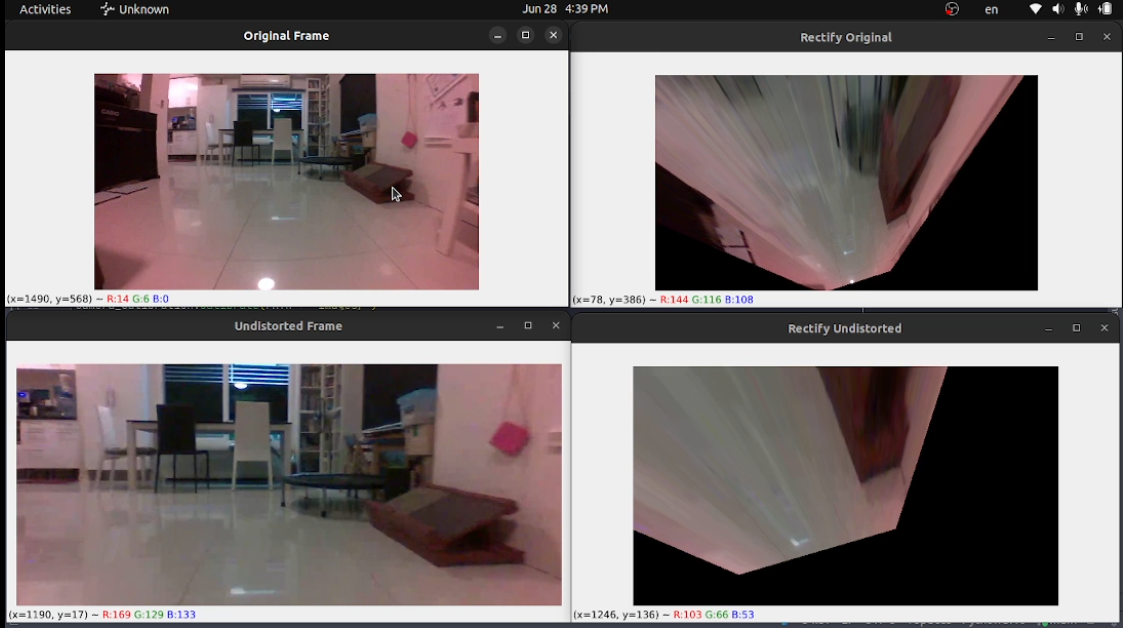
\includegraphics[scale=0.3]{images/Matt_vidoe_result.png}
	\end{figure}
	\begin{lstlisting}
# calibrate_camera.py		
import glob
import cv2 as cv
import numpy as np


class CameraCalibration:
    camera_mtx = None
    distortion_coefficient = None
    rotation_vectors = None
    translation_vectors = None

    # Define the dimensions of checkerboard
    __CHECKERBOARD = (6, 9)
    __criteria = (cv.TERM_CRITERIA_EPS + cv.TERM_CRITERIA_MAX_ITER, 30, 0.001)

    # Create vector to store vectors of 3D points for each checkerboard image
    __obj_points = []

    # Create vector to store vectors of 2D points for each checkerboard image
    __img_points = []

    # Define the world coordinates for 3D points
    __obj_point = np.zeros((1, __CHECKERBOARD[0] * __CHECKERBOARD[1], 3), dtype=np.float32)
    __obj_point[0, :, :2] = np.mgrid[0:__CHECKERBOARD[0], 0:__CHECKERBOARD[1]].T.reshape(-1, 2)
    __prev_img_shape = None

    __img = None
    __gray = None

    def __init__(self, file_name=None):
        if file_name is not None:
            self.read_calibration_file(file_name)

    def calibrate(self, file_path):
        images = glob.glob(file_path + "*.jpg")

        for f_name in images:
            self.__img = cv.imread(f_name)
            self.__gray = cv.cvtColor(self.__img, cv.COLOR_BGR2GRAY)

            # Find the checkerboard corners
            ret, corners = cv.findChessboardCorners(self.__gray, self.__CHECKERBOARD, cv.CALIB_CB_ADAPTIVE_THRESH
                                                    + cv.CALIB_CB_FAST_CHECK + cv.CALIB_CB_NORMALIZE_IMAGE)

            # If the desired number of corner are detected
            if ret:
                self.__obj_points.append(self.__obj_point)

                # Refining pixel coordinates for given 2D points.
                corners2 = cv.cornerSubPix(self.__gray, corners, (9, 9), (-1, -1), self.__criteria)

                self.__img_points.append(corners2)

                # Draw and display the corners
                self.__img = cv.drawChessboardCorners(self.__img, self.__CHECKERBOARD, corners2, True)

            cv.imshow('img', self.__img)
            cv.waitKey(30)
        cv.destroyAllWindows()

        # Calibrate the camera
        ret, self.camera_mtx, self.distortion_coefficient, self.rotation_vectors, self.translation_vectors = \
            cv.calibrateCamera(self.__obj_points, self.__img_points, self.__gray.shape[::-1], None, None)

    def write_calibration_file(self, file_name):
        file_storage = cv.FileStorage(file_name, cv.FILE_STORAGE_WRITE)

        if not file_storage.isOpened():
            return False

        file_storage.write("MTX", self.camera_mtx)
        file_storage.write("DIST", self.distortion_coefficient)
        for i in range(10):
            file_storage.write("R" + str(i), self.rotation_vectors[i])
            file_storage.write("T" + str(i), self.translation_vectors[i])
        file_storage.release()

        return True

    def read_calibration_file(self, file_name):
        file_storage = cv.FileStorage(file_name, cv.FILE_STORAGE_READ)
        if not file_storage.isOpened():
            return False

        self.camera_mtx = file_storage.getNode("MTX").mat()
        self.distortion_coefficient = file_storage.getNode("DIST").mat()
        r_vectors = tuple()
        t_vectors = tuple()
        for i in range(10):
            r_vectors += (file_storage.getNode("R" + str(i)).mat(),)
            t_vectors += (file_storage.getNode("T" + str(i)).mat(),)
        self.rotation_vectors = r_vectors
        self.translation_vectors = t_vectors
        file_storage.release()

        return True
	\end{lstlisting}

	\begin{lstlisting}
# homography.py		
import cv2 as cv
import numpy as np


class Homography:
    mat_h = np.zeros((3, 3))
    width_out: int
    height_out:  int
    c_points: int
    a_points: list = []

    __point = (-1, -1)
    __pts = []
    __var = 0
    __drag = 0
    __mat_final = np.array([])
    __mat_result = np.array([])

    def __init__(self, homography_file=None):
        self.c_points = 0
        if homography_file is not None:
            self.read(homography_file)

    def read(self, homography_file: str):
        file_storage = cv.FileStorage(homography_file, cv.FILE_STORAGE_READ)
        if not file_storage.isOpened():
            return False

        self.c_points = 0
        for i in range(4):
            point = file_storage.getNode("aPoints" + str(i))
            self.a_points.append(point.mat())
            self.c_points += 1

        self.mat_h = file_storage.getNode("matH").mat()
        self.width_out = int(file_storage.getNode("widthOut").real())
        self.height_out = int(file_storage.getNode("heightOut").real())
        file_storage.release()
        return True

    def write(self, homography_file):
        file_storage = cv.FileStorage(homography_file, cv.FILE_STORAGE_WRITE)
        if not file_storage.isOpened():
            return False

        for i in range(4):
            file_storage.write("aPoints" + str(i), self.a_points[i])

        file_storage.write("matH", self.mat_h)
        file_storage.write("widthOut", self.width_out)
        file_storage.write("heightOut", self.height_out)
        file_storage.release()

        return True

    def __draw_circle_and_line(self, x, y):
        self.__mat_result = self.__mat_final.copy()
        self.__point = (x, y)

        if self.__var >= 1:
            cv.line(self.__mat_result, self.__pts[self.__var - 1], self.__point, (0, 255, 0, 255), 2)
        cv.circle(self.__mat_result, self.__point, 2, (0, 255, 0), -1, 8, 0)
        cv.imshow("Source", self.__mat_result)

    def __mouse_handler(self, event, x, y, flags, param):
        if self.__var >= 4:
            return

        if event == cv.EVENT_LBUTTONDOWN:
            self.__drag = 1
            self.__draw_circle_and_line(x, y)

        if event == cv.EVENT_LBUTTONUP and self.__drag:
            self.__drag = 0
            self.__pts.append(self.__point)
            self.__var += 1
            self.__mat_final = self.__mat_result.copy()

            if self.__var >= 4:
                cv.line(self.__mat_final, self.__pts[0], self.__pts[3], (0, 255, 0, 255), 2)
                cv.fillConvexPoly(self.__mat_final, np.array(self.__pts, dtype=np.int32), (0, 120, 0, 20))
            cv.imshow("Source", self.__mat_final)

        if self.__drag:
            self.__draw_circle_and_line(x, y)

    def calculate(self, file_name):
        mat_pause_screen = np.array([])
        mat_frame_capture = np.array([])
        key = -1

        # --------------------- [STEP 1: Make video capture from file] ---------------------
        # Open video file
        video_capture = cv.VideoCapture(file_name)
        if not video_capture.isOpened():
            print("ERROR! Unable to open input video file ", file_name)
            return False

        width = video_capture.get(cv.CAP_PROP_FRAME_WIDTH)
        height = video_capture.get(cv.CAP_PROP_FRAME_HEIGHT)
        ratio = 640.0 / width
        dim = (int(width * ratio), int(height * ratio))

        while key < 0:
            # Get the next frame
            _, mat_frame_capture = video_capture.read()
            if mat_frame_capture is None:
                break

            mat_frame_display = cv.resize(mat_frame_capture, dim)

            cv.imshow("Original", mat_frame_display)
            key = cv.waitKey(30)

        # --------------------- [STEP 2: pause the screen and show an image] ---------------------
            if key >= 0:
                mat_pause_screen = mat_frame_capture
                self.__mat_final = mat_pause_screen.copy()

        cv.destroyAllWindows()

        # --------------------- [STEP 3: use mouse handler to select 4 points] ---------------------
        if mat_frame_capture is not None:
            self.__var = 0
            self.__pts.clear()
            cv.namedWindow("Source", cv.WINDOW_GUI_NORMAL)
            cv.setMouseCallback("Source", self.__mouse_handler)
            cv.imshow("Source", mat_pause_screen)
            cv.waitKey(0)
            cv.destroyWindow("Source")

            if len(self.__pts) == 4:
                src = np.array(self.__pts).astype(np.float32)

                reals = np.array([
                    (800, 800),
                    (1000, 800),
                    (1000, 1000),
                    (800, 1000)
                ], dtype=np.float32)

        # --------------------- [STEP 4: Calculate Homography] ---------------------
                homography_matrix = cv.getPerspectiveTransform(src, reals)

        # --------------------- [STEP 4: Calculate Homography] ---------------------
                self.mat_h = homography_matrix
                self.c_points = 0
                for i in range(4):
                    self.a_points.append(src[i])
                    self.c_points += 1
                self.width_out = int(width)
                self.height_out = int(height)

                return True
        else:
            return False
	\end{lstlisting}

	\begin{lstlisting}
# main.py		
import sys
import cv2 as cv
from calibrate_camera import CameraCalibration
from homography import Homography

PATH = "../../../../Data/Lab03/robot/"
VIDEO_FILE = "robot.mp4"

# Calibrate the camera
camera_calibration = CameraCalibration()
camera_calibration.calibrate(PATH + "images/")
camera_calibration.write_calibration_file("camera_calibration.yml")

print("Camera matrix: ", camera_calibration.camera_mtx)
print("Distortion coefficient: ", camera_calibration.distortion_coefficient)
print("Rotation vectors: ", camera_calibration.rotation_vectors)
print("Translation vectors: ", camera_calibration.translation_vectors)

# Calculate homography
homography_data = Homography()
homography_data.calculate(PATH + VIDEO_FILE)
homography_data.write("homography.yml")

print("Estimated Homography matrix: \n", homography_data.mat_h)

# Show undistorted and rectify images
video_capture = cv.VideoCapture(PATH + VIDEO_FILE)
if not video_capture.isOpened():
    print("ERROR! Unable to open video file ", VIDEO_FILE)
    sys.exit()
width = video_capture.get(cv.CAP_PROP_FRAME_WIDTH)
height = video_capture.get(cv.CAP_PROP_FRAME_HEIGHT)
ratio = 600.0 / width
dim = (int(width * ratio), int(height * ratio))

duration = 0
while True:
    _, frame = video_capture.read()
    if frame is None:
        break

    # Undistorted and Cropped the frame
    h, w = frame.shape[:2]
    new_camera_mtx, roi = cv.getOptimalNewCameraMatrix(camera_calibration.camera_mtx,
                                                       camera_calibration.distortion_coefficient,
                                                       (w, h), 1, (w, h))
    undistorted_frame = cv.undistort(frame, camera_calibration.camera_mtx,
                                     camera_calibration.distortion_coefficient)
    x, y, w, h = roi
    cropped_undistorted_frame = undistorted_frame[y:y+h, x:x+w]

    # Show the original and undistorted frames
    cv.namedWindow("Original Frame", cv.WINDOW_NORMAL | cv.WINDOW_KEEPRATIO | cv.WINDOW_GUI_EXPANDED)
    cv.imshow("Original Frame", frame)
    cv.namedWindow("Undistorted Frame", cv.WINDOW_NORMAL | cv.WINDOW_KEEPRATIO | cv.WINDOW_GUI_EXPANDED)
    cv.imshow("Undistorted Frame", cropped_undistorted_frame)

    # Show the rectified original and undistorted frames
    result_original = cv.warpPerspective(frame, homography_data.mat_h,
                                         (int(homography_data.width_out), int(homography_data.height_out)),
                                         cv.INTER_LINEAR)
    result_undistorted = cv.warpPerspective(cropped_undistorted_frame, homography_data.mat_h,
                                            (int(homography_data.width_out), int(homography_data.height_out)),
                                            cv.INTER_LINEAR)
    cv.namedWindow("Rectify Original", cv.WINDOW_NORMAL | cv.WINDOW_KEEPRATIO | cv.WINDOW_GUI_EXPANDED)
    cv.imshow("Rectify Original", result_original)
    cv.namedWindow("Rectify Undistorted", cv.WINDOW_NORMAL | cv.WINDOW_KEEPRATIO | cv.WINDOW_GUI_EXPANDED)
    cv.imshow("Rectify Undistorted", result_undistorted)

    cv.waitKey(duration)
    if duration == 0:
        duration = 30
cv.destroyAllWindows()
	\end{lstlisting}

	\subsection{Do you get better result?}
	The better result is acheived by undistorting the image because distorition in the images especially radial distorition are removed from the images.
	
\end{document}